\newcommand{\figureLCDCharPlayer}[1]{
  \def\lang{\detokenize{#1}}
  \def\langRu{\detokenize{ru}}
  \def\langEn{\detokenize{en}}
  \def\figureCaption{XXX: No translation.}
  \ifx \lang\langRu
  \def\figureCaption{
    Изображение игрока.
  }
  \fi
  \ifx \lang\langEn
  \def\figureCaption{
    Image of a player.
  }
  \fi
\begin{figure}[ht]
  \centering
  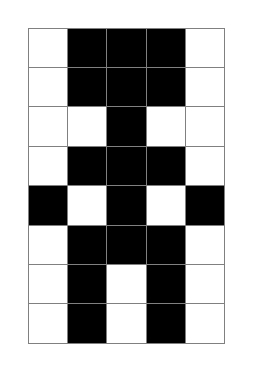
\begin{tikzpicture}
    %% 0
    \fill[black] (-2.0, 0) rectangle (-0.5, -1.0);
    %% 2
    \fill[black] (-1.0, -1.0) rectangle (-1.5, -1.5);
    %% 3
    \fill[black] (-0.5, -1.5) rectangle (-2.0, -2.0);
    %% 4
    \fill[black] (-2.0, -2.0) rectangle (-2.5, -2.5);
    \fill[black] (-1.5, -2.0) rectangle (-1.0, -2.5);
    \fill[black] (-0.5, -2.0) rectangle (-0.0, -2.5);
    %% 5
    \fill[black] (-0.5, -2.5) rectangle (-2.0, -3.0);
    %% 6
    \fill[black] (-2.0, -3.0) rectangle (-1.5, -3.5);
    \fill[black] (-1.0, -3.0) rectangle (-0.5, -3.5);
    %% 7
    \fill[black] (-2.0, -3.5) rectangle (-1.5, -4.0);
    \fill[black] (-1.0, -3.5) rectangle (-0.5, -4.0);
    \draw[step=0.5cm,gray,very thin] (-2.5, -4.0) grid (0, 0);
  \end{tikzpicture}
  \caption{\figureCaption}
  \label{fig:game-dev-char-symbol-example}
\end{figure}
}
